\documentclass{beamer}
\usepackage{listings}
\usepackage{xcolor}

%\setbeameroption{show only notes}

% must use LuaLaTeX to compile with non-standard fonts
\usepackage{fontspec}
\setmonofont[
    Path        = /Users/mackenziemorgan/Library/Fonts/,
    Extension   = .ttf,
    Scale       = 0.7
]{FiraCode-Regular}
\setmainfont[
    Extension      = .ttc,
    Ligatures      = TeX
]{GillSans}

\usetheme{Madrid}
\useinnertheme{circles}
\definecolor{Axiosblue}{HTML}{2257da} 
\usecolortheme[named=Axiosblue]{structure}

% from https://gist.github.com/m1dnight/95f405c9c41f208a16df0a68b6ccbfda
\definecolor{commentgreen}{RGB}{2,112,10}
\definecolor{eminence}{RGB}{108,48,130}
\definecolor{weborange}{RGB}{255,165,0}
\definecolor{frenchplum}{RGB}{129,20,83}

\lstdefinelanguage{elixir}{
    morekeywords={case,catch,def,do,else,false,%
        use,alias,receive,timeout,defmacro,defp,%
        for,if,import,defmodule,defprotocol,%
        nil,defmacrop,defoverridable,defimpl,%
        super,fn,raise,true,try,end,with,%
        unless},
    otherkeywords={<-,->, |>, \%\{, \}, \{, \, (, )},
    sensitive=true,
    morecomment=[l]{\#},
    morecomment=[n]{/*}{*/},
    morecomment=[s][\color{purple}]{:}{\ },
    morestring=[s][\color{orange}]"",
    commentstyle=\color{commentgreen},
    keywordstyle=\color{eminence},
    stringstyle=\color{red},
	basicstyle=\ttfamily,
	breaklines,
	showstringspaces=false,
	frame=l
}
	
\lstset{xleftmargin=2em,frame=single,framexleftmargin=0em,numberstyle=\footnotesize\ttfamily}


%Information to be included in the title page:
\title{Dealing with a Monster Ecto Query}
\author{Mackenzie Morgan}
\institute{Axios}
\date{Elixir Wizards Conference 2021}

\begin{document}

\frame{\titlepage}

\begin{frame}
\frametitle{About Me}
A year ago, I learned Elixir because we launched the Axios mobile app and immediately crashed Apollo.
\pause

Every morning.
\pause

At 6AM.
\pause

I'm not a morning person.
\end{frame}

\note{
To be clear, I'm not the one who did the initial port to Elixir. There were contractors involved. I picked it up and started extending it, and it generally worked great...except for this one query.
}

\begin{frame}
\frametitle{The problem}
	A single complex query with a lot of ORs is responsible for the majority of our database load.
	\pause
	
	And the biggest day in US political news is next week.
	\pause
	
	(the presidential election)
\end{frame}

\note{
Moving as much computation into the database and out of the code as possible is a pretty common piece of advice for optimization. You know, sort and limit on the database instead of in code, so the database has less stuff to return to start with.

This is a story of when to refactor the opposite direction and how a couple Elixir features helped.

If you've worked for a newspaper during a presidential election,  you know that everyone is on call that night, and users are hammering the servers, trying to find out who won.}

\begin{frame}
\frametitle{Context}
  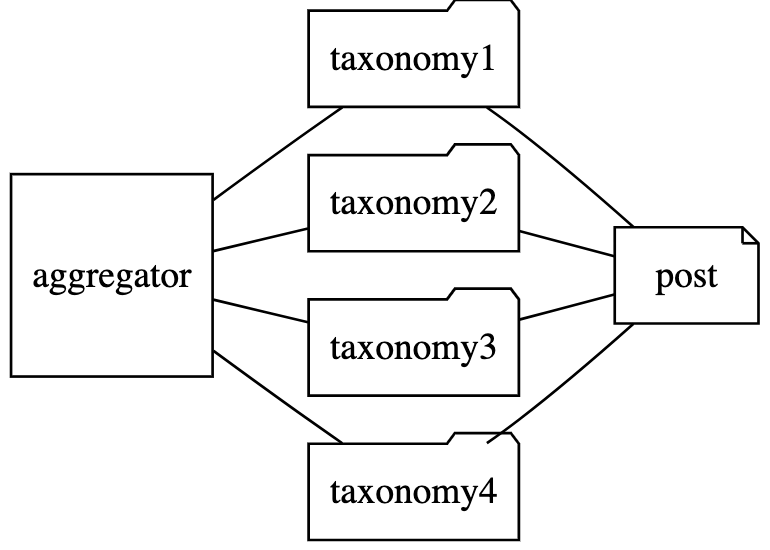
\includegraphics[height=0.7\textheight]{data_model.png}
\end{frame}

\note{It's pretty standard for a CMS to support multiple taxonomies,  like categories AND tags.  We depended, at the time, on 4 separate taxonomies to decide what you see when you load up the Axios mobile app.}

\begin{frame}
	\frametitle{Starting code}
	\lstinputlisting[language=elixir]{original_code.ex}
\end{frame}

\note{We knew from AWS stats that this was the toughest query. I've simplified it here to leave out date ranges, sorting, etc, but the original Postgres analyze result was a cost of 3614 and 8 millisecond execution time. Let's walk through refactoring this to be super-fast.}


\begin{frame}
\frametitle{Break it down}
\pause
	What if we do 4 smaller queries?
	\pause
	\lstinputlisting[language=elixir]{step_1.ex}
	\pause
	Written out 4 times,  once for each taxonomy
\end{frame}

\note{That alone is gets us down to Postgres saying its cost is 16 and execution time is 0.125ms, so we're on the right track. But it's no prettier than the original.}

\begin{frame}
\frametitle{Not DRY enough}
\pause
	What if we take advantage of atoms and the pin operator?
	\pause
	\lstinputlisting[language=elixir]{step_2.ex}
	\pause
	And call it 4 times,  once for each taxonomy
\end{frame}

\note{Thanks to the ability to pass around atoms and dereference them inside Ecto queries, we can at least abstract that query into a function. But we still have to write 4 calls to that function, which is still a little ugly.}

\begin{frame}
\frametitle{Just a little further}
\pause
	What if we use Elixir's famed concurrency?
	\pause
	\begin{columns}
		\begin{column}{0.3\textwidth}
		    \lstinputlisting[language=elixir]{final_code_left.ex}
		\end{column}
		\begin{column}{0.6\textwidth}
		    \lstinputlisting[language=elixir]{final_code.ex}
		\end{column}
	\end{columns}
\end{frame}

\note{Hey, there we go. Now, we can make all 4 queries at the same time, just passing in the list of taxonomies. That's really nice if you ever need more taxonomies. (Guess what? I'm now using 5.)}

\begin{frame}
\frametitle{Results}
	\begin{itemize}
		\item DB CPU utilization: 50\% $\rightarrow$ 40\% (-20\%)
\pause
		\item Postgres analyze cost: 3614 $\rightarrow$ 16
		\item Postgres analyze execution time: 8.424ms $\rightarrow$ 0.125ms $\times$ 4 $=$ 0.5ms
\pause
		\item Max requests per second: 700\%
\pause
		\item Stress-free Election Night
	\end{itemize}
\end{frame}

\note{This isn't the first newspaper I've worked for. I remember the stress of mid-term elections, smooth sailing for the presidential was a nice change. And look, our day-to-day database CPU usage went down by 20\% too.}

\begin{frame}
\frametitle{Find Me Online}
  \begin{itemize}
    \item \textbf{Twitter:} @maco\_nix
    \item \textbf{GitHub:} @maco
    \item \textbf{Homepage:} mackenzie.morgan.name
    \item \textbf{Elixir Slack:} @maco
  \end{itemize}
\end{frame}

\end{document}
